\appendix
\chapter{Testarea fiabilității modelului CLIENT-SERVER}
\section{Script}

\scriptsize \begin{verbatim}
#!/bin/bash

# seconds_EPOCH.sh

while read line

do
    echo $(date +%s) ":" $line;
done
\end{verbatim}
\par
\par ---------------------------------------------------------------------------------------
\par 
\scriptsize \begin{verbatim}
#!/bin/bash

# RUN_TESTS.sh

#!/bin/bash

telnetClients=10
rm ./*.out

echo "INCHIDEM SERVERUL ..."
kill -9 `pidof java` 
echo "START SERVER .... in 3 secunde "
java server &
sleep 3s
echo "OK" 

for ((1; i<=$telnetClients; ++i )) ; 
do
    fileName="./file_$i.out"
    telnet localhost 8080 | ./seconds_EPOCH.sh | tee -a $fileName &
done
\end{verbatim}

\section{Server de test}

\scriptsize \begin{lstlisting}
import java.net.ServerSocket;
import java.net.Socket;
import java.io.BufferedReader;
import java.io.IOException;
import java.io.InputStreamReader;
import java.io.PrintStream;
import java.util.ArrayList;

class SClient extends Thread {

    private Socket 		socket;
    private Integer 		serverId;
    private BufferedReader	istream;
    private PrintStream 	ostream;
    private boolean 		keepRunning;
    private static ArrayList<SClient> allServers = new ArrayList<SClient>();

    @SuppressWarnings("unused")
	private SClient() {
	// blocat
    }
	

    public SClient(Socket socket, Integer id) throws IOException {
		
	this.socket = socket;
	this.serverId = id;
	this.istream = new BufferedReader(new InputStreamReader(this.socket.getInputStream()));
	this.ostream = new PrintStream(socket.getOutputStream());
	this.keepRunning = true;
		
	allServers.add( this );
    }

    public void sendResponse(String response) {
	this.ostream.println(response);
    }
	
    private String getRequest() throws IOException {
	String line = "";

	try{
	    int c = 0;
	    while(((char)c)!='\n'){
		c= this.istream.read();
		line = line+(char)c;
		if(c==-1){
		    this.keepRunning = false;
		    break;
		}
	    }
	} catch (Exception e) {
	    e.printStackTrace();
	    this.keepRunning = false;
	}
		
	return line;
    }

    @Override
	public void run() {
	super.run();

	while(keepRunning) {
			
	    String text = "";
	    try {
		text = this.getRequest();
	    } catch (IOException e) {
		e.printStackTrace();
		text = "EROARE";
	    }
			
	    if ( text.contains("quit") || text.contains("exit") )
		{
		    System.exit(0);
		}

	    try{
			
		if ( allServers.size() >= 1 ) {
					
		    for(SClient user : allServers) {
			if(user!=null) {
			    user.sendResponse(text);
			}
		    }
		}
				
	    } catch (Exception e){
		e.printStackTrace();
		this.sendResponse("\nEROARE");
	    }
	}

	try {
	    this.socket.close();
	} catch (IOException e) {
	    e.printStackTrace();
	}
    }

}

/*

              serverul de test

*/

public class server {
	
    public static void main(String[] args){
		
	/*
	 *  in asteptarea clientilor
	 */
	int serverId=1;
	ServerSocket serverSocket;
	try {
	    serverSocket = new ServerSocket(8080);
	    for(;;){
		Socket s = serverSocket.accept();
		System.out.print("\nNew server [id="+serverId+"]");
		/*
		 *  client nou
		 */
		Thread t = new SClient(s, serverId);
		serverId++;
		t.start();
	    }
	} catch (IOException e) {
	    e.printStackTrace();
	}

    }
}

\end{lstlisting}


\subsection{Rezultate}
\par La verificarea diferențelor de timp la primirea datelor de către programele client cu comanda \textbf{ diff <fisier1> <fisier2> }. Testul este disponibil pentru verificare directorul ”Teste/ApendixA” în arhiva GIT a lucrării. Descărcarea se poate face cu comanda \textbf{git clone  https://github.com/gabrielchmod777/virtualWorldVRML-CLIENT.git}.

\par Testul este efectuat cu succes.
\newpage
\chapter{Îcărcarea dinamică a claselor în JAVA}

\scriptsize \begin{verbatim}

#!/bin/bash

#
# check.sh -> assert în SHELL
#
typeset -i tests_run=0
function try { this="$1"; }
trap 'printf "$0: exit code $? on line $LINENO\nFAIL: $this\n"; exit 1' ERR
function assert {
        let tests_run+=1
        [ "$1" = "$2" ] && { echo -n "."; return; }
        printf "\nFAIL: $this\n'$1' != '$2'\n"; exit 1
}

try "test diff"
# ...
assert $1 $2

echo; echo "PASS: $tests_run tests run"

\end{verbatim}

\scriptsize \begin{verbatim}
#!/bin/bash

#
# runTest.sh
#

echo 'Start test\n'
echo '-------------------------'
echo 'Testeaza -> Add 1 1'
v1=`java ApendixB Add 1 1`
./check.sh 2 $v1
echo '-------------------------'
echo 'Testeaza -> Add 5 1'
v1=`java ApendixB Add 5 1`
./check.sh 6 $v1
echo '-------------------------'
echo 'Testeaza -> Sub 1 1'
v1=`java ApendixB Sub 1 1`
./check.sh 0 $v1
echo '-------------------------'
echo 'Testeaza -> Sub 5 1'
v1=`java ApendixB Sub 5 1`
./check.sh 4 $v1
echo '-------------------------'
echo 'Testeaza -> Add 10 10'
v1=`java ApendixB Add 10 10`
./check.sh 20 $v1
echo '-------------------------'
echo 'Testeaza -> Sub 10 11'
v1=`java ApendixB Sub 10 11`
./check.sh -1 $v1
echo '-------------------------'
echo 'Testeaza -> Sub 19 3'
v1=`java ApendixB Sub 19 3`
./check.sh 16 $v1
echo '-------------------------'
echo 'Testeaza -> Add 101 10'
v1=`java ApendixB Add 101 10`
./check.sh 111 $v1
echo '-------------------------'
echo 'Testeaza -> Sub 0 3'
v1=`java ApendixB Sub 0 3`
./check.sh -3 $v1
echo '-------------------------'
echo 'Testeaza -> Sub 1 1'
v1=`java ApendixB Sub 1 1`
./check.sh 0 $v1
echo '-------------------------'
echo 'Stop test\n'

\end{verbatim}

\newpage

\scriptsize \begin{verbatim}

public interface Operatie {
	void evaluate(Integer a, Integer b);
}
++++++++++++++++++++++++++++++++++++++++++++++++++++++++++++++++++++++++++++++++++

public class Add implements Operatie {
	@Override
	public void evaluate(Integer a, Integer b) {
		Integer x = a + b;
		System.out.print(Integer.toString(x));
	}
}

++++++++++++++++++++++++++++++++++++++++++++++++++++++++++++++++++++++++++++++++++

public class Sub implements Operatie {
	@Override
	public void evaluate(Integer a, Integer b) {
		Integer x = a - b;
		System.out.print(Integer.toString(x));
	}
}

++++++++++++++++++++++++++++++++++++++++++++++++++++++++++++++++++++++++++++++++++

public class ApendixB {

	public static void main(String[] args) {

		if ( args.length < 3 )
		{
			System.out.println("Eroare");
		}
		
		String classNameToBeLoaded = args[0];
		Integer a = Integer.parseInt(args[1]);
		Integer b = Integer.parseInt(args[2]);

		ClassLoader myClassLoader = ApendixB.class.getClassLoader();
		try {
			Class<?> myClass = myClassLoader.loadClass(classNameToBeLoaded);
			Object instance = myClass.newInstance();
			
			if("Add".equals(classNameToBeLoaded)) {
				((Add)instance).evaluate(a, b);
			} else if("Sub".equals(classNameToBeLoaded)) {
				((Sub)instance).evaluate(a, b);
			} else  {
				System.out.println("Eroare");
			}
			
			
		} catch (ClassNotFoundException | InstantiationException | IllegalAccessException e) {
			System.out.println("Eroare");
		}
		
	}

}

\end{verbatim}

\newpage

\scriptsize \begin{verbatim}

Start test\n
-------------------------
Testeaza -> Add 1 1
.
PASS: 1 tests run
-------------------------
Testeaza -> Add 5 1
.
PASS: 1 tests run
-------------------------
Testeaza -> Sub 1 1
.
PASS: 1 tests run
-------------------------
Testeaza -> Sub 5 1
.
PASS: 1 tests run
-------------------------
Testeaza -> Add 10 10
.
PASS: 1 tests run
-------------------------
Testeaza -> Sub 10 11
.
PASS: 1 tests run
-------------------------
Testeaza -> Sub 19 3
.
PASS: 1 tests run
-------------------------
Testeaza -> Add 101 10
.
PASS: 1 tests run
-------------------------
Testeaza -> Sub 0 3
.
PASS: 1 tests run
-------------------------
Testeaza -> Sub 1 1
.
PASS: 1 tests run
-------------------------
Stop test\n

\end{verbatim}
\newpage
\subsection*{SERVER - Diagrama UML completă}
\begin{figure}[h]
    \centering
    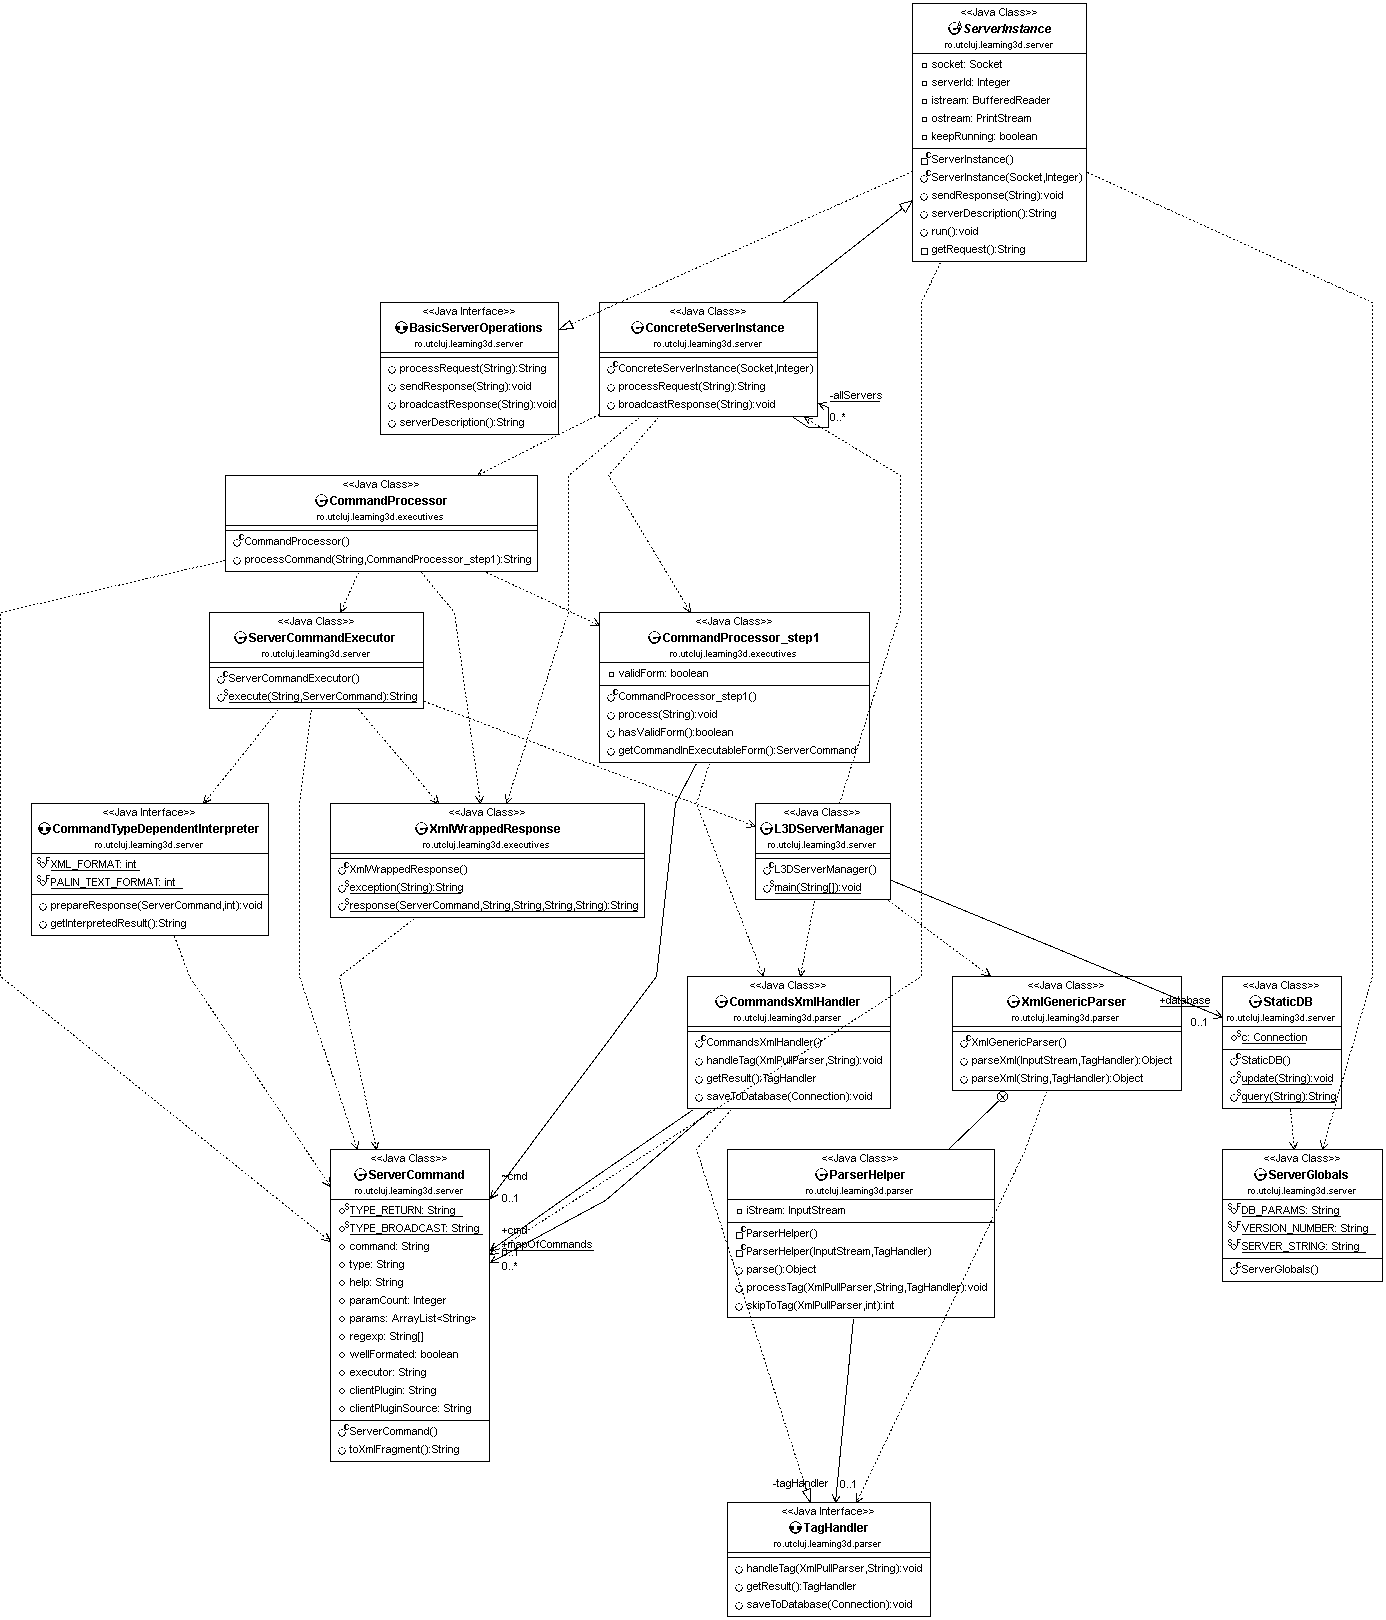
\includegraphics[scale=0.35]{fsunml}
    \caption{Server - diagrama UML completă}
    \label{fig:imagSrvUML}
\end{figure}
\newpage
\chapter{Iconuri grafice utilizate pentru nodurile VRML în lucrarea ”The Inventor Mentor”}
\begin{figure}[h]
    \centering
    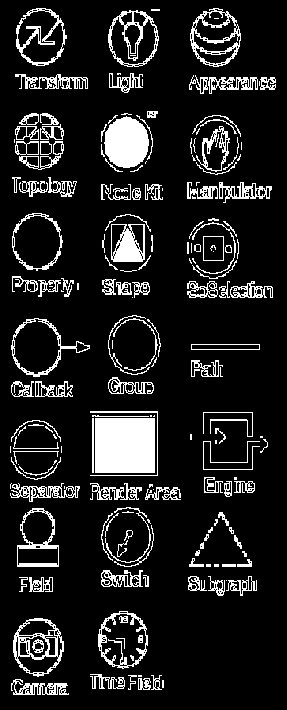
\includegraphics[scale=0.5]{nodvrml}
    \caption{Noduri VRML}
    \label{fig:imagSrvUML}
\end{figure}